\documentclass[tikz,border=1cm]{standalone}
\usetikzlibrary{patterns,matrix,backgrounds}
\usepackage{amsmath,amssymb}
\begin{document}
	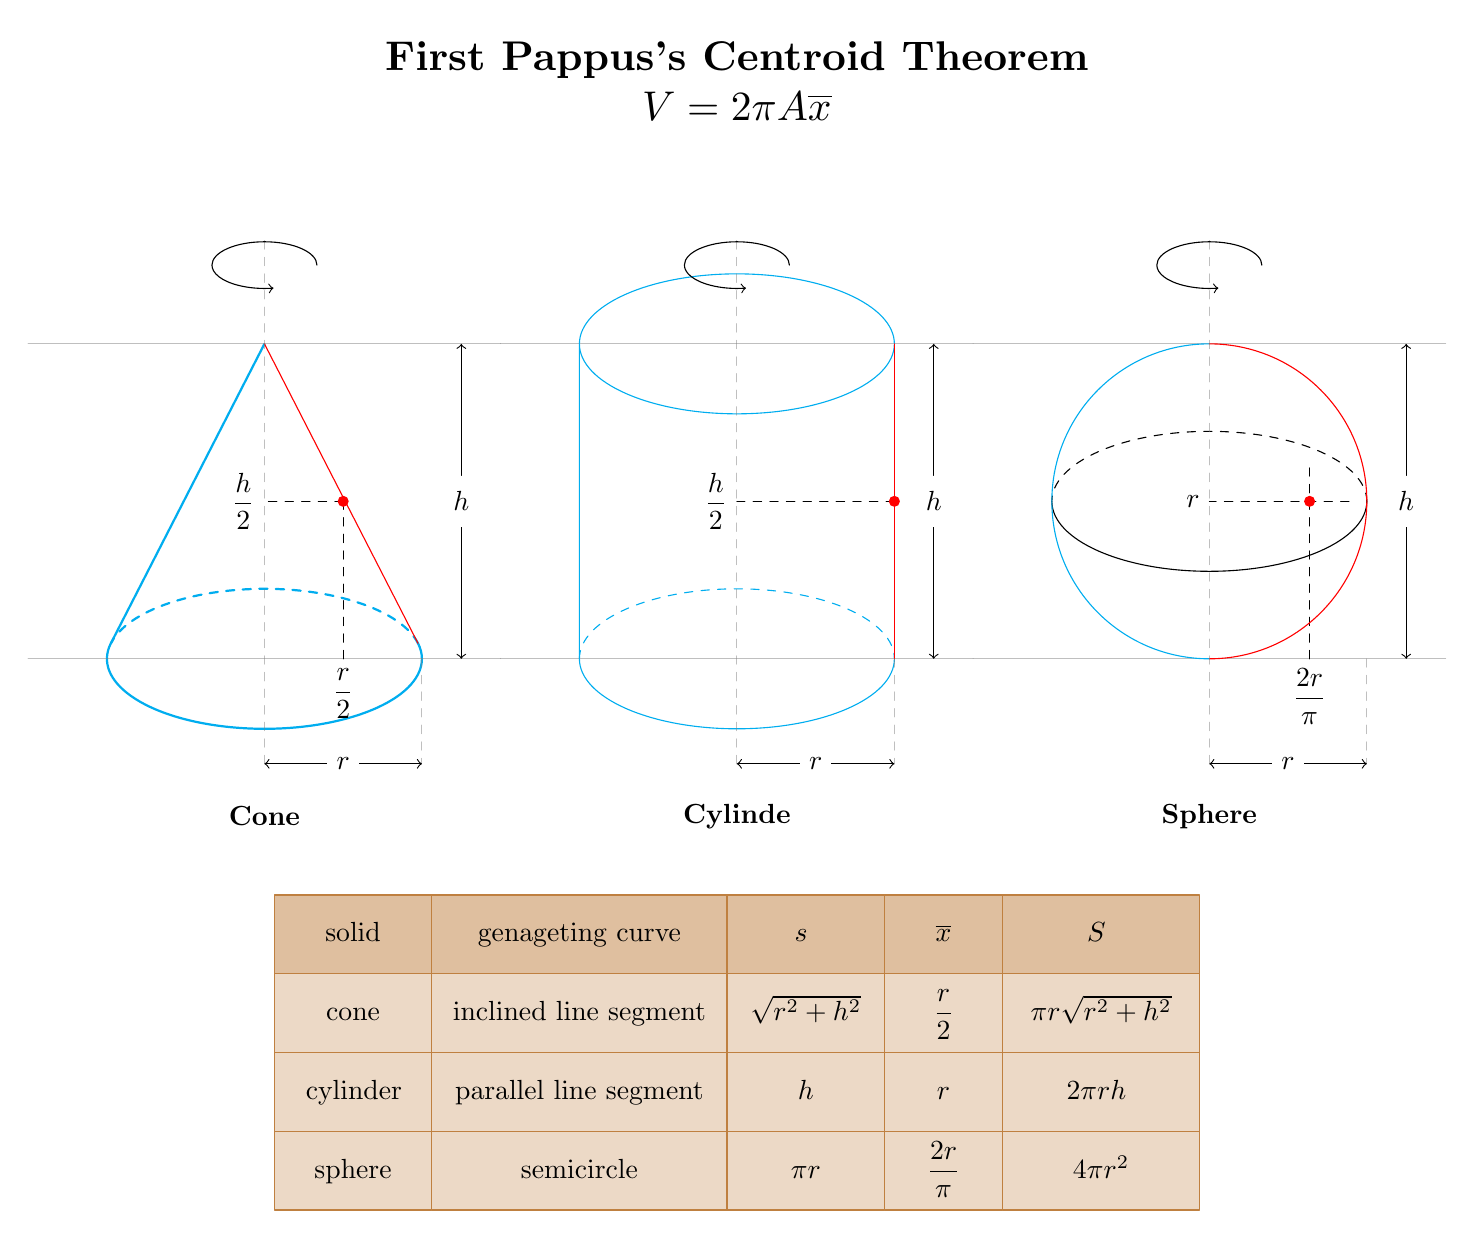
\begin{tikzpicture}[line join=round, line cap=round]
		\def\a{2}% Bán trục lớn
		\def\b{\a/2.25}% Bán trục bé
		\pgfmathsetmacro{\h}{2*\a}% Chiều cao
		\pgfmathsetmacro{\xc}{2*\a/(pi)}
		\def\d{3*\a}
		\tikzset{chuthich/.pic={
				\draw [dashed, gray,opacity=0.5](0,-\h/3)--([shift={(0,\h/3)}]0,\h)(\a,0)--(\a,-\h/3);
				\draw[->](\a/3,1.25*\h)arc(0:280:{\a/3} and {\b/3});
				\draw[<->,shift={(1.25*\a,0)}](0,0)--(90:\h)node[pos=0.5,circle,fill=white]{$h$};
				\draw[<->](0,-\h/3)--(\a,-\h/3)node[pos=0.5,fill=white]{$r$};}}
		%%Hình nón=======nodeone
		\tikzset{nodeone/.pic={
				\pgfmathsetmacro{\t}{asin(\b/\h)}
				\coordinate (M) at ({\a*cos(\t)}, {\b*sin(\t)});
				\coordinate (N) at ({-\a*cos(\t)}, {\b*sin(\t)});
				\coordinate (O) at (0,0);
				\coordinate (A) at (\a,0);
				\coordinate (B) at (-\a,0);
				\draw[dashed,cyan,thick] (M) arc(\t:{180-\t}:{\a} and {\b});
				\draw [cyan,thick](0,\h)--(N) arc({180-\t}:{360+\t}:{\a} and {\b});
				\draw [gray,opacity=0.5](-1.5*\a,0)--(1.5*\a,0)(-1.5*\a,\h)--(1.5*\a,\h);
				\draw[dashed,thin](\a/2,0)node[below]{$\dfrac{r}{2}$}--(\a/2,\h/2)(\a/2,\h/2)--(0,\h/2)node[left]{$\dfrac{h}{2}$};
				\fill[red](\a/2,\h/2)circle(2pt);
				\draw[red](M)--(0,\h);
				\path (0,-\h/2)node{\textbf{Cone}};}}
		%%%Hình trụ: nodetwo================
		\tikzset{nodetwo/.pic={
				\draw[dashed,cyan](-\a,0)arc(180:0: {\a} and {\b});
				\draw [gray,opacity=0.5](-1.5*\a,0)--(1.5*\a,0)(-1.5*\a,\h)--(1.5*\a,\h);
				\draw[cyan](-\a,\h)arc(-180:180: {\a} and {\b})--++(-90:\h)arc(180:360: {\a} and {\b});
				\draw[red](\a,0)--(\a,\h);
				\draw[dashed,thin](\a,\h/2)--(\a/2,\h/2)--(0,\h/2)node[left]{$\dfrac{h}{2}$};
				\fill[red](\a,\h/2)circle(2pt);
				\path (0,-\h/2)node{\textbf{Cylinde}};}}
		%%Hình cầu: nodethree==================
		\tikzset{nodethree/.pic={
				\coordinate (A) at (\a,0);
				\coordinate (B) at (-\a,0);
				\coordinate (O) at (0,0);
				\draw [gray,opacity=0.5](-1.5*\a,0)--(1.5*\a,0)(-1.5*\a,\h)--(1.5*\a,\h);
				\draw(\a,\h/2)arc(0:-180: {\a} and {\b});
				\draw[dashed](\a,\h/2)arc(0:180: {\a} and {\b});
				\draw[dashed,thin](\xc,0)node[below]{$\dfrac{2r}{\pi}$}--([shift={(0,0.5)}]\xc,\h/2)([shift={(0.5,0)}]\xc,\h/2)--(0,\h/2)node[left]{$r$};
				\draw[cyan](O)arc(-90:-270: {\h/2} and {\h/2});
				\draw[red](O)arc(270:450: {\h/2} and {\h/2});
				\fill[red](\xc,\h/2)circle(2pt);
				\path (0,-\h/2)node{\textbf{Sphere}};}}
		\path (0,0)pic{nodeone}pic{chuthich}(\d,0)pic{nodetwo}pic{chuthich}(2*\d,0)pic{nodethree}pic{chuthich};
		\path (current bounding box.north)++(0,\a)
		node[scale=1.5,align=center]
		{\bfseries \textbf{First Pappus's Centroid Theorem}\\
			$V=2\pi A\overline{x}$};
		\begin{scope}[shift={(\d,-1.25*\h)}]
			\matrix[matrix of nodes,
			row sep=-\pgflinewidth,
			column sep=-\pgflinewidth,
			nodes={draw=brown,text height=1.5ex,text depth=.25ex,minimum height=1cm},
			column 1/.style={minimum width=\a cm,text width=1.2cm,align=left},
			column 2/.style={minimum width=3.75cm,text width=3.5cm,align=left},
			column 3/.style={minimum width=2cm,align=center},
			column 4/.style={minimum width=1.5cm,align=center},
			column 5/.style={minimum width=2.5cm,align=center},
			row 1/.style={nodes={fill=brown!50,align=center}},
			row 2/.style={nodes={fill=brown!30,align=center}},
			row 3/.style={nodes={fill=brown!30,align=center}},
			row 4/.style={nodes={fill=brown!30,align=center}}
			]{
				solid & genageting curve& $s$ &$\overline{x}$& $S$ \\
				cone & inclined line segment& $\sqrt{r^2+h^2}$&$\dfrac{r}{2}$&$\pi r\sqrt{r^2+h^2}$\\
				cylinder & parallel line segment & $h$&$r$& $2\pi rh$ \\
				sphere & semicircle & $\pi r$&$\dfrac{2r}{\pi}$&$4\pi r^2$\\
			};
		\end{scope}
	\end{tikzpicture}

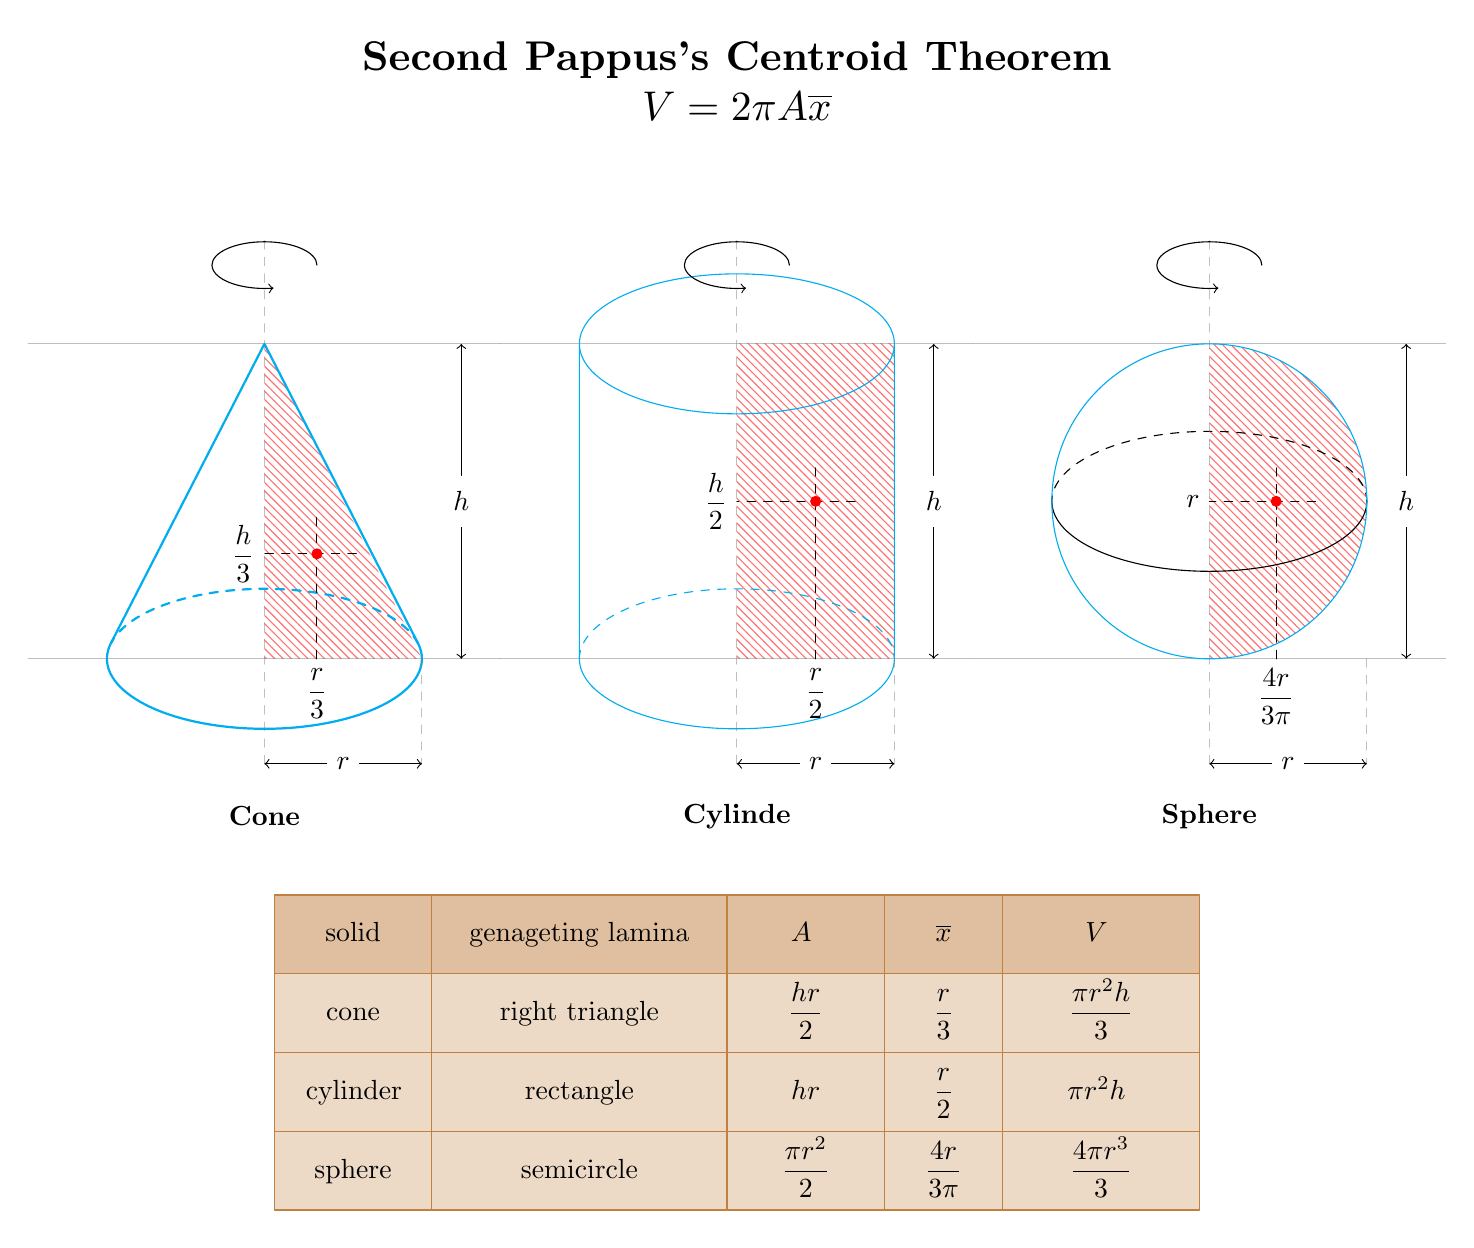
\begin{tikzpicture}[line join=round, line cap=round]
	\def\a{2}% Bán trục lớn
	\def\b{\a/2.25}% Bán trục bé
	\pgfmathsetmacro{\h}{2*\a}% Chiều cao
	\pgfmathsetmacro{\xc}{4*\a/(3* pi)}
	\def\d{3*\a}
	\tikzset{chuthich/.pic={
			\draw [dashed, gray,opacity=0.5]([shift={(0,-\h/3)}]O)--([shift={(0,\h/3)}]0,\h)(\a,0)--(\a,-\h/3);
			\draw[->](\a/3,1.25*\h)arc(0:280:{\a/3} and {\b/3});
			\draw[<->,shift={(1.25*\a,0)}](0,0)--(90:\h)node[pos=0.5,circle,fill=white]{$h$};
			\draw[<->](0,-\h/3)--(\a,-\h/3)node[pos=0.5,fill=white]{$r$};}}
	%%Hình nón=======nodeone
	\tikzset{nodeone/.pic={
			\pgfmathsetmacro{\t}{asin(\b/\h)}
			\coordinate (M) at ({\a*cos(\t)}, {\b*sin(\t)});
			\coordinate (N) at ({-\a*cos(\t)}, {\b*sin(\t)});
			\coordinate (O) at (0,0);
			\coordinate (A) at (\a,0);
			\coordinate (B) at (-\a,0);
			\fill[pattern=north west lines,pattern color=pink!60!red](0,0)--(\a,0)--(0,\h)--cycle;
			\draw[dashed,cyan,thick] (M) arc(\t:{180-\t}:{\a} and {\b});
			\draw [cyan,thick](0,\h)--(N) arc({180-\t}:{360+\t}:{\a} and {\b})--(0,\h);
			\draw [gray,opacity=0.5](-1.5*\a,0)--(1.5*\a,0)(-1.5*\a,\h)--(1.5*\a,\h);
			\draw[dashed,thin](\a/3,0)node[below]{$\dfrac{r}{3}$}--([shift={(0,0.5)}]\a/3,\h/3)([shift={(0.5,0)}]\a/3,\h/3)--(0,\h/3)node[left]{$\dfrac{h}{3}$};
			\fill[red](\a/3,\h/3)circle(2pt);
			\path (0,-\h/2)node{\textbf{Cone}};}}
	%%%Hình trụ: nodetwo================
	\tikzset{nodetwo/.pic={
			\coordinate (A) at (\a,0);
			\coordinate (B) at (-\a,0);
			\coordinate (O) at (0,0);
			\fill[pattern=north west lines,pattern color=pink!60!red](O)rectangle(\a,\h);
			\draw[dashed,cyan](B)arc(180:0: {\a} and {\b});
			\draw [gray,opacity=0.5](-1.5*\a,0)--(1.5*\a,0)(-1.5*\a,\h)--(1.5*\a,\h);
			\draw[cyan](-\a,\h)arc(-180:180: {\a} and {\b})--++(-90:\h)arc(180:360: {\a} and {\b})--(\a,\h);
			\draw[dashed,thin](\a/2,0)node[below]{$\dfrac{r}{2}$}--([shift={(0,0.5)}]\a/2,\h/2)([shift={(0.5,0)}]\a/2,\h/2)--(0,\h/2)node[left]{$\dfrac{h}{2}$};
			\fill[red](\a/2,\h/2)circle(2pt);
			\path (0,-\h/2)node{\textbf{Cylinde}};}}
	%%Hình cầu: nodethree==================
	\tikzset{nodethree/.pic={
			\coordinate (A) at (\a,0);
			\coordinate (B) at (-\a,0);
			\coordinate (O) at (0,0);
			\fill[pattern=north west lines,pattern color=pink!60!red](O)arc(-90:90: {\h/2})--cycle;
			\draw [gray,opacity=0.5](-1.5*\a,0)--(1.5*\a,0)(-1.5*\a,\h)--(1.5*\a,\h);
			\draw(\a,\h/2)arc(0:-180: {\a} and {\b});
			\draw[dashed](\a,\h/2)arc(0:180: {\a} and {\b});
			\draw[dashed,thin](\xc,0)node[below]{$\dfrac{4r}{3\pi}$}--([shift={(0,0.5)}]\xc,\h/2)([shift={(0.5,0)}]\xc,\h/2)--(0,\h/2)node[left]{$r$};
			\draw[cyan](O)arc(-90:-450: {\h/2} and {\h/2});
			\fill[red](\xc,\h/2)circle(2pt);
			\path (0,-\h/2)node{\textbf{Sphere}};}}
	\path (0,0)pic{nodeone}pic{chuthich}(\d,0)pic{nodetwo}pic{chuthich}(2*\d,0)pic{nodethree}pic{chuthich};
	\path (current bounding box.north)++(0,\a)
	node[scale=1.5,align=center]
	{\bfseries \textbf{Second Pappus's Centroid Theorem}\\
		$V=2\pi A\overline{x}$};
	\begin{scope}[shift={(\d,-1.25*\h)}]
		\matrix[matrix of nodes,
		row sep=-\pgflinewidth,
		column sep=-\pgflinewidth,
		nodes={draw=brown,text height=1.5ex,text depth=.25ex,minimum height=1cm},
		column 1/.style={minimum width=\a cm,text width=1.2cm,align=left},
		column 2/.style={minimum width=3.75cm,text width=3.5cm,align=left},
		column 3/.style={minimum width=2cm,align=center},
		column 4/.style={minimum width=1.5cm,align=center},
		column 5/.style={minimum width=2.5cm,align=center},
		row 1/.style={nodes={fill=brown!50,align=center}},
		row 2/.style={nodes={fill=brown!30,align=center}},
		row 3/.style={nodes={fill=brown!30,align=center}},
		row 4/.style={nodes={fill=brown!30,align=center}}
		]{
			solid & genageting lamina& $A$ &$\overline{x}$& $V$ \\
			cone & right triangle& $\dfrac{hr}{2}$&$\dfrac{r}{3}$&$\dfrac{\pi r^2h}{3}$\\
			cylinder & rectangle & $hr$&$\dfrac{r}{2}$&$\pi r^2h$ \\
			sphere & semicircle & $\dfrac{\pi r^2}{2}$&$\dfrac{4r}{3\pi}$&$\dfrac{4\pi r^3}{3}$\\
		};
	\end{scope}
\end{tikzpicture}
\end{document}